\section{Symmetrie}
Das Wort Symmetrie ist sehr alt und hat sich seltsamerweise von seinem
ursprünglichen griechischen Wort
\(\mathrm{\Sigma\upsilon\mu\mu\varepsilon\tau\rho\iota\alpha}\)
\footnote{\emph{Symmetr\'ia}: ein gemeinsames Mass habend, gleichmässig,
verhältnismässig} fast nicht verändert. In der Alltagssprache mag es ein
locker definierter Begriff sein, aber in der Mathematik hat Symmetrie eine sehr
präzise Bedeutung.
\begin{definition}[Symmetrie]
	Ein mathematisches Objekt wird als symmetrisch bezeichnet, wenn es unter einer
	bestimmten Operation invariant ist.
\end{definition}
Die intuitivsten Beispiele kommen aus der Geometrie, daher werden wir mit
einigen geometrischen Beispielen beginnen. Wie wir jedoch später sehen werden,
ist das Konzept der Symmetrie eigentlich viel allgemeiner.  

\begin{figure}
	\centering
	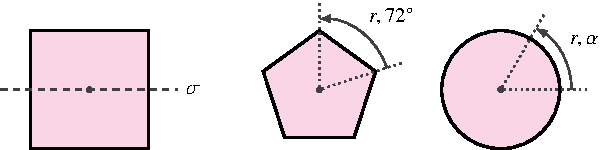
\includegraphics{papers/punktgruppen/figures/symmetric-shapes}
	\caption{
		Beispiele für geometrisch symmetrische Formen.
		\label{fig:punktgruppen:geometry-example}
	}
\end{figure}

\subsection{Geometrische Symmetrien}

In Abbildung \ref{fig:punktgruppen:geometry-example} haben wir einige Formen,
die offensichtlich symmetrisch sind.  Zum Beispiel hat das Quadrat eine Gerade,
an deren es gespiegelt werden kann, ohne sein Aussehen zu verändern.
Regelmässige Polygone mit \(n\) Seiten sind auch gute Beispiele, um eine
diskrete Rotationssymmetrie zu veranschaulichen, was bedeutet, dass eine
Drehung um einen Punkt um einen bestimmten Winkel \(360^\circ/n\) die Figur
unverändert lässt.  Das letzte Beispiel auf der rechten Seite ist eine
unendliche Rotationssymmetrie. Sie wird so genannt, weil es unendlich viele
Werte für \(\alpha \in \mathbb{R}\) gibt, die die Form unverändert lassen.  Ein
Objekt kann mehr als nur eine Symmetrie aufweisen.  Als Beispiel, kann das
Quadrat in Abbildung \ref{fig:punktgruppen:geometry-example} nicht nur um
\(\sigma\) sondern auch Diagonal gespiegelt werden oder um \(90^\circ\) gedreht
werden.  Fasst man die möglichen Symmetrien zusammen, entsteht eine
Symmetriegruppe.

\begin{definition}[Symmetriegruppe]
	Sei \(g\) eine umkehrbare Operation, die ein mathematisches Objekt
	unverändert lässt.  Bei einer anderen Operation \(h\) definieren wir die
	Komposition \(h\circ g\) als die Anwendung der Operationen nacheinander. Alle
	Operationen bilden unter Komposition eine Gruppe, die Symmetriegruppe genannt
	wird.
\end{definition} % ich lese diese  Definition ein wenig holprig, vieleicht können wir sie zusammen anschauen

Ausserdem benötigen wir zur Bildung einer Gruppe ein neutrales Element, das wir
mit \(\mathds{1}\) bezeichnen. Die Anwendung der neutralen Operation ist
gleichbedeutend damit, alles unverändert zu lassen. \(\mathds{1}\) ist auch
äquivalent dazu, eine Operation anzuwenden und sie dann rückgängig zu machen
(ihre Umkehrung anzuwenden).
Die Definition der Symmetriegruppe ist mit der Kompositionsoperation gegeben,
es wird aber auch oft als Multiplikation geschrieben. Das liegt daran, dass
manchmal die Zusammensetzung algebraisch durch eine Multiplikation berechnet
wird. Die Verwendung einer multiplikativen Schreibweise ermöglicht es, einige
Ausdrücke kompakter zu schreiben, z.B. durch Verwendung von Potenzen \(r^n =
r\circ r \circ \cdots r\circ r\) für eine wiederholte Komposition. 

\begin{definition}[Zyklische Untergruppe, Erzeuger]
	Sei \(g\) ein Element einer Symmetriegruppe \(G\). Alle möglichen
	Kompositionen von \(g\) und \(g^{-1}\) bilden eine sogenannte zyklische
	Untergruppe von \(G\), und \(g\) wird ihr Erzeuger genannt. Die von \(g\)
	erzeugte Untergruppe \(\langle g \rangle = \left\{ g^k : k \in \mathbb{Z}
	\right\}\) wird mit spitzen Klammern bezeichnet.
\end{definition}
\begin{beispiel}
	Um die Syntax zu verstehen, betrachten Sie eine durch \(a\) erzeugte Gruppe
	\(G = \langle a \rangle\).  Das bedeutet, dass \(G\) die Elemente \(a, aa,
	aaa, \ldots\) sowie \(a^{-1}, a^{-1}a^{-1}, \ldots\) und ein neutrales
	Element \(\mathds{1} = aa^{-1}\) enthält.
\end{beispiel}
\begin{beispiel}
	Nun zu einem sinnvolleren Beispiel, wir können das \(n\)-Gon Beispiel
	formalisieren.  Bezeichnen wir mit \(r\) eine Drehung im Gegenuhrzeigersinn
	von \(360^\circ/n\) um einen Punkt.  Diese Definition reicht aus, um die
	gesamte Symmetriegruppe
	\[
		C_n = \langle r \rangle
			= \left\{\mathds{1}, r, r^2, \ldots, r^{n-1}\right\}
	\]
	der Drehungen eines \(n\)-Gons zu erzeugen. Das liegt daran, dass wir durch
	die mehrfache Verwendung von \(r\) jeden Winkel erzeugen k\"onnen, der die
	Rotationssymmetrie bewahrt. In ähnlicher Weise, aber weniger interessant die
	Reflexionssymmetriegruppe \(\langle\sigma\rangle\) enthält nur
	\(\left\{\mathds{1}, \sigma\right\}\), weil \(\sigma^2 = \mathds{1}\).
\end{beispiel}

Wenn wir diese Idee nun erweitern, können wir mit einem Erzeugendensystemen
komplexere Strukturen aufbauen.

\begin{definition}[Erzeugendensysteme]
	% please fix this unreadable mess
	Jede disktrete Gruppe kann durch eines oder mehrere ihrer Elemente generiert
	werden.  Wir lassen \(g_1, g_2, \ldots, g_n\) erzeugenden Elemente einer
	Symmetriegruppe sein.  Da es mehrere Erzeuger gibt, müssen auch die
	sogenannte Definitionsgleichungen gegeben werden, die die
	Multiplikationstabelle vollständig definieren. Die Gleichungen sind ebenfalls
	in den Klammern angegeben. Die erzeugende Elementen zusammen mit der
	Definitionsgleichungen bauen ein Erzeugendensysteme.
\end{definition}
\begin{beispiel}
	Wir werden nun alle Symmetrien eines \(n\)-Gons beschreiben, was bedeutet,
	dass wir die Operationen \(r\) und \(\sigma\) kombinieren. Die
	Definitionsgleichungen sind \(r^n = \mathds{1}\), \(\sigma^2 =
	\mathds{1}\) und \((\sigma r)^2 = \mathds{1}\).
	Die ersten beiden sind ziemlich offensichtlich. Die letzte wird oft auch als
	Inversion bezeichnet, weil die Anwendung von \(\sigma r\) dasselbe ist wie
	das Ziehen einer Linie von einem Punkt, die durch den Ursprung geht, und das
	Verschieben des Punktes auf die andere Seite des Nullpunkts. Wenn man das
	zweimal macht, geht man zurück zum Anfangspunkt.
	Daraus ergibt sich die so genannte Diedergruppe 
	\begin{align*}
		D_n &= \langle r, \sigma : r^n = \sigma^2 = (\sigma r)^2 = \mathds{1} \rangle \\
			&= \left\{
					\mathds{1}, r, \ldots, r^{n-1}, \sigma, \sigma r, \ldots, \sigma r^{n-1}
			\right\}.
	\end{align*}
\end{beispiel}

Die Symmetrieoperationen, die wir bis jetzt besprochen haben, haben immer
mindestens einen Punkt gehabt, der wieder auf sich selbst abgebildet wird. Im
Fall der Rotation war es der Drehpunkt, bei der Spiegelung die Punkte der
Spiegelachse. Dies ist jedoch keine Voraussetzung für eine Symmetrie, da es
Symmetrien gibt, die jeden Punkt zu einem anderen Punkt verschieben können.
Diesen Spezialfall, bei dem mindestens ein Punkt unverändert bleibt, nennt man
Punktsymmetrie.
\begin{definition}[Punktgruppe]
	Wenn es einen Punkt gibt, der von jeder Gruppenoperation unverändert gelassen
	wird, sagt man, dass die Symmetriegruppe eine Punktgruppe ist.
\end{definition}

\subsection{Algebraische Symmetrien}
Wir haben nun unseren Operationen Symbole gegeben, mit denen es tatsächlich
möglich ist, Gleichungen zu schreiben.  Die folgende Frage ist dann, ob wir
bereits mathematische Objekte haben, mit denen wir Gleichungen schreiben, die
sich auf die gleiche Weise verhalten. Die Antwort lautet natürlich ja.  Um es
formaler zu beschreiben, werden wir einige Begriffe einführen.
\begin{definition}[Gruppenhomomorphismus]
	Seien \(G\) und \(H\) Gruppe mit unterschiedlicher Operation \(\diamond\)
	bzw.  \(\star\). Ein Homomorphismus\footnote{ Für eine ausführlichere
	Diskussion siehe \S\ref{buch:grundlagen:subsection:gruppen} im Buch.} ist
	eine Funktion \(f: G \to H\), so dass für jedes \(a, b \in G\) gilt
	\(f(a\diamond b) = f(a) \star f(b)\).  Man sagt, dass der Homomorphismus
	\(f\) \(G\) in \(H\) transformiert.
\end{definition}
\begin{beispiel}
	Die Rotationssymmetrie des Kreises \(C_\infty\), mit einem unendlichen
	Kontinuum von Werten \(\alpha \in \mathbb{R}\), entspricht perfekt dem
	komplexen Einheitskreis. Der Homomorphismus \(\phi: C_\infty \to \mathbb{C}\)
	ist durch die Eulersche Formel \(\phi(r) = e^{i\alpha}\) gegeben.
\end{beispiel}

\begin{definition}[Darstellung einer Gruppe]
	Die Darstellung einer Gruppe ist ein Homomorphismus, der eine Symmetriegruppe
	auf eine Menge von Matrizen abbildet.
	\[
		\Phi: G \to \operatorname{GL}_n(\mathbb{R}).
	\]
	Äquivalent kann man sagen, dass ein Element aus der Symmetriegruppe auf einen
	Vektorraum \(V\) wirkt, indem man definiert \(\Phi : G \times V \to V\).
\end{definition}
\begin{beispiel}
	Die Elemente \(r^k \in C_n\), wobei \(0 < k < n\), stellen abstrakt eine
	Drehung von \(2\pi k/n\) um den Ursprung dar. Die mit der Matrix 
	\[
		\Phi(r^k) = \begin{pmatrix}
			\cos(2\pi k/n) & -\sin(2\pi k/n) \\
			\sin(2\pi k/n) &  \cos(2\pi k/n)
		\end{pmatrix}
	\]
	definierte Funktion von \(C_n\) nach \(O(2)\) ist eine Darstellung von
	\(C_n\). In diesem Fall ist die erste Gruppenoperation die Komposition und
	die zweite die Matrixmultiplikation. Man kann überprüfen, dass \(\Phi(r^2
	\circ r) = \Phi(r^2)\Phi(r)\).
\end{beispiel}

%% TODO: title / fix continuity
% Um das Konzept zu illustrieren, werden wir den umgekehrten Fall diskutieren:
% eine Symmetrie, die keine Punktsymmetrie ist, die aber in der Physik sehr
% nützlich ist, nämlich die Translationssymmetrie.  Von einem mathematischen
% Objekt \(U\) wird gesagt, dass es eine Translationssymmetrie \(Q(x) = x + a\)
% hat, wenn es die Gleichung 
% \[
% 	U(x) = U(Q(x)) = U(x + a),
% \]
% für ein gewisses \(a\), erfüllt. Zum Beispiel besagt das erste Newtonsche
% Gesetz, dass ein Objekt, auf das keine Kraft einwirkt, eine
% zeitranslationsinvariante Geschwindigkeit hat, d.h. wenn \(\vec{F} = \vec{0}\)
% dann \(\vec{v}(t) = \vec{v}(t + \tau)\).

% \subsection{Sch\"onflies notation} 

% vim:ts=2 sw=2 spell spelllang=de:
